

% Hence I rely on the hypothesis that the Zone is integrated to an execution framework by hooking asynchronous code submission to the framework and binding that code to the Zone.


% Given the multity of asynchronous frameworks in the Java ecosystem selecting one 


% In conclusion, this small overview of the asynchronous world shows that in Java, one cannot assume

% Threads used as worker in pools are unaware of when they switch tasks and have no vision...
% Therefore, realizing a Zone 

% In Java, unlike dart and javascript there is no unique imposed asynchronous model but lots of frameworks built on top of natives threads.



% Hence, the Zone developed in this project aim to integrate with any approach. The tool must stay consistent regardless of the asynchronous framework. Single threaded, multi threaded, callbacks, events or promises.

% This multiplicity brings a constraint on
% As long as you can 

% As we will see in the next chapter, the Zone need a hook on asynchronous task submission

% In term of integration, the use of thread pools make it impossible to realize a thread-level hook
% The final solution is proposed into two decoupled parts: the integration and the functionalities. The integration, shortly discussed in chapter \label{ch:asyncworld} simply requires that the asynch

% Thus the present model aims for general and composable features, allowing to build specific behaviors.

% \section{Application Needs}

% What the model need to fill following requirements.

% \begin{itemize}
% \item include input and output to the zoned code
% \item generals hooks that allow error handling implementation as well as on-the-fly Zone definition.
% \item resolution of the contextual ambiguity in asynchronous error handling
% \end{itemize}

% Last elements introduce need of uniform behavior between synchronous and asynchronous execution.
% That is the real point of exec context.

\chapter{The Zone}
\label{ch:zone}

The Zone is an execution context associated to a code block. It represents the asynchronous extension of a scope. Like a scope, the Zone can contain other Zones.

%Any code executed or asynchronoulsy submitted in a Zone stays in that Zone. This guarantees asynchronous consistency. A Zone can contain another Zone, as a scope enclnoses inner scopes. The Zone defines key-value bindings, the equivalent of lexically scoped values. Similarily, the Zone can overload 

The primordial purpose of Zones is to answer the lack of context persistency when submitting asynchronous task. Zones allow to store key-value bindings and persist across asynchronous execution. Hence, they make it possible to share information between asynchronous executions. Because the key-value bindings may be shared by concurrent executions, they must stay immutable to avoid race conditions. However, it is still possible to locally add more key-value bindings by creating a new Zone with additional bindings. It is safe since concurrent executions won't be affected by the local context modification. Furthermore, it is still possible in Java to bypass this limitation, modifiying the \emph{content} of immutable references.

The Zone is intended to provide a context across asynchronous executions. It specifies constant values accessible through context (Zone values), task to execute when entering (cross-in hook) or exiting (cross-out hook) a Zone and hooks around synchronous and asynchronous task execution. Those around hooks make it possible to manipulate the tasks that get executed inside the Zone. While they are not essential to the concept of Zone itself, the opportunity to implement them naturally appears in a Zone implementation since it is a Zone requirement (see next section). The Zone can then simply make these hooks accessible on its interface.

\section{Model}

As illustrated in figure \ref{fig:zpn}, the Zone can be understood as an extension to Perti net that allows to capture the tokens flow.

\begin{figure}
  \centering
  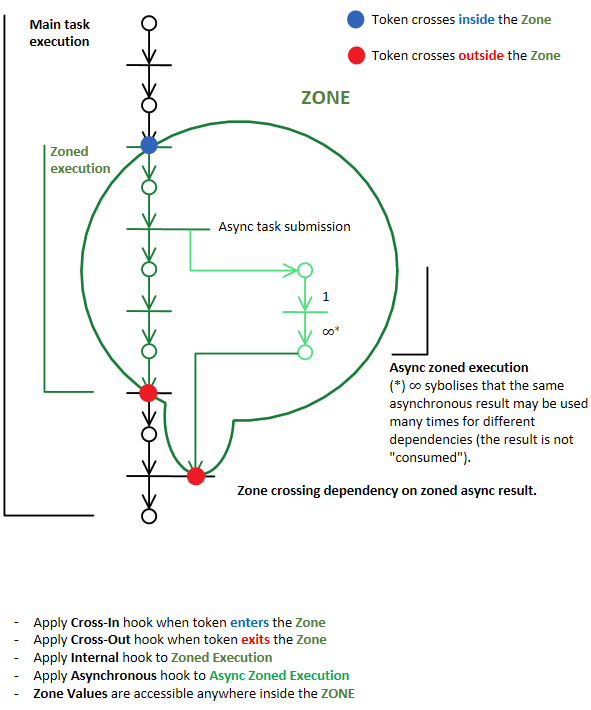
\includegraphics[width=\textwidth]{zone-pn}
  \caption{Zone on Petri net}
  \label{fig:zpn}
\end{figure}

More formally, given a Petri net $PN = (P, T, F)$ with $P$ the set of places, $T$ the set of transitions and $F$ the set of flows from $P$ to $T$ or $T$ to $P$: $F \subseteq (P \times T) \cup (T \times P)$, a Zone $Z$ is a subset $Z \subseteq P$ such that

$$\forall Z_1, Z_2 (Z_1 \cap Z_2 \neq \emptyset) \Rightarrow [(Z_1 \subseteq Z_2) \lor (Z_2 \subseteq Z_1)] $$

$$\forall Z_1, Z_2 \exists Z_0 \text{ s.t. } Z_1 \subseteq Z_0 \land Z_2 \subseteq Z_0 $$

Which more simply means: there exists a \emph{root} Zone enclosing all Zones and Zones can contain other Zones, but cannot intersect otherwise (figure \ref{fig:zinter}).

\begin{figure}[h]
  \centering
  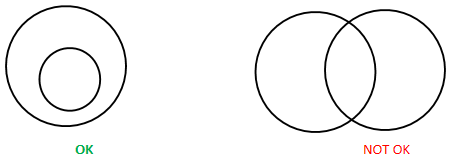
\includegraphics[width=\textwidth]{zone-intersect}
  \caption{Zone intersection}
  \label{fig:zinter}
\end{figure}

Additionally, the Zone defines key-value bindings that are accessible from any place inside the Zone and crossing hooks that are triggered whenever a token crosses a Zone boundary.

The Zone identifies a crossing event when a token moves between two places that do not belong to the same Zones (see crossing algorithm). For more liberty in the crossing hooks, tokens may carry nothing (void tokens) an error (error tokens) or the result of a zoned task (result tokens). Programmatically, the tokens are implemented as simple objects containing a result, an error value or nothing.

In order to know which Zone originated a token, they are wrapped as zoned tokens. A zoned token is simply a tuple containing a Token and its origin Zone.

Operations on token while crossing Zone boundaries are described by the Zone's crossing hooks.
The presence of around hooks defined in the Zone allows even more capabilities. Howver, unlike the crossing hooks, these around hooks are closer to an implementation feature than a primary effect of the model.

\section{Terminology}

In order to ease further discussion and presentation of the Zone, this section gives a small glossary of the essential terms used in the Zone.


\paragraph{Task} represents the very general concept of ``something the program has to do''. More formally, a task is a procedure with some input and zero or one output. For example, a Runnable is a task with no input, no output. A method call is a task with method's arguments as input and method's return value as output.

\paragraph{Zoned Token} A zoned token is a tuple containing a token with its origin Zone. Zoned tokens are used as input to the cross resolution algorithm (see cross resolution section).

\paragraph{Zoned Task} A zoned Task is the result of binding a task to a Zone. A Zoned task behaves like a task but accepts and return only zoned tokens. For instance a task expressed in Java by
\begin{lstlisting}
Function<T, U> task;
\end{lstlisting}
Is associated to a zoned task represented by
\begin{lstlisting}
Function<ZonedToken<T>, ZonedToken<U>> zonedTask;
\end{lstlisting}

\paragraph{Zone Stack} is the stack of all enclosing zones at a given point of the program execution. Innermost Zone is considered to be at the top of the Zone Stack. If no Zone is defined, the current Zone is considered to be the default root Zone. For example :

\begin{lstlisting}
(new ZoneA()).run(() -> {
  /*
   * Zone stack here is:
   * ZoneA, ROOT_Zone
   */
   (new ZoneB()).run(() -> {
     /*
      * Zone stack here is:
      * ZoneB, ZoneA, ROOT_ZONE
      */
   });
});
/*
 * Zone stack here is back to:
 * ROOT_ZONE
 */
\end{lstlisting}

\section{Cross Resolution}

The crossing principle is the original feature of the Zone. The base mechanism is simple. Value outputted by zoned tasks are \emph{zoned tokens}. When the value of a zoned token is used, it is extracted to the current Zone triggering the crossed Zones crossing hook on the fly.

Multiple cases can occur with crossing mechanisms. Especially in the Java implementation, where it is possible to keep and carry around references to already bound tasks, a token extraction can occur in unexpected contexts. Rather than relying on visibility restrictions to prevent such unusual cases to occur, the cross resolution defines how the model behaves under such circumstances.

For better understanding, keep in mind that at the bottom of every single Zone stack, there is the Root Zone. The Root Zone can be seen as the Zone with no hooks and values enclosing the whole program.

In the given code examples, \lstinline{new Zone()} creates a Zone whose parent is the enclosing Zone. For instance:

\begin{lstlisting}
Zone zone1 = new Zone();
Zone zone2;
zone1.run(() -> {
  // inside zone1
  zone2 = new Zone();
});

assert(zone1.getParent() == ROOT_ZONE);
assert(zone2.getParent() == zone1);
\end{lstlisting}

The cross resolution algorithm always applies to three parameters :

\begin{enumerate}
\item The source Zone (src)
\item The destination Zone (dst)
\item The crossing Token (tkn)
\end{enumerate}

The crossing token is \emph{not} a zoned token. Zoned token used by the framework provides the source Zone of the cross resolution algorithm. The destination Zone is the current zone of the extraction and the crossing token.

\begin{enumerate}
\item Collect the Zone stack of the source Zone and the destination Zone to get the source stack and the destination stack.
\item Eliminate the common bottom part of the stacks. Recall that every Zone is a (indirect) child of the Root Zone, hence both stacks have at lesast one Zone in common. The idea of this step is to find the closest common enclosing Zone of src and dst: the \emph{join Zone}.
\item Cross out the rest of the source stack in top-down order with tkn. This means calling each crossing hooks of the crossed Zone with the crossing token as argument.
\item Cross in the rest of the destination stack in down-top order with tkn.
\end{enumerate}

Let's see some concrete example of crossing executions.

\subsection*{Base case}

The common case of zoned execution is running code in a child Zone.

\begin{lstlisting}
// current Zone = some Zone

(new Zone()).run(() -> {
  // current Zone = new Zone

  // do zoned stuff here
});
\end{lstlisting}

when teh code zoned in new Zone starts, the cross algorithm executes in a very simple configuration.

\begin{tabular}{| l | l |}
\hline
\textbf{Source Zone} & Some Zone \\ \hline
\textbf{Destination Zone} & New Zone \\ \hline
\textbf{Join Zone} & Some Zone \\ \hline
\end{tabular}

Since the join Zone is the source Zone, the left source stack after step 2 is empty. Step 3 of the algorithm has no effect. No cross-out hook is applied, only one cross-in, of the destination Zone, is executed.

When the code zoned in new Zone ends, the cross algorithm executes in the dual configuration, still simple:

\begin{tabular}{| l | l |}
\hline
\textbf{Source Zone} & New Zone \\ \hline
\textbf{Destination Zone} & Some Zone \\ \hline
\textbf{Join Zone} & Some Zone \\ \hline
\end{tabular}

The join Zone is still the source Zone, but the left destination stack is emptied by step 2. Step 3 executes one cross out (from the source Zone), step 4 executes no cross In. To summarize, in this case, a cross in is executed when entering the new Zone, a cross out is executed when entering the old Zone. So far, so good.

\subsection*{Running in parent Zone from child Zone}

This is a simple case that allows to see that running code in a Zone does not necessarily implies crossing in.

\begin{lstlisting}
// keeps reference to parent Zone
Zone parent = new Zone();

parent.run(() -> {
  // inside Zone parent
  Zone child = new Zone();
  child.run(() -> {
    // inside Zone child

    // this is the point of interes
    parent.run(() -> {
      // Zoned code here !!
    });
  });
});
\end{lstlisting}

When the code zoned in parent (at the point of interest) starts, the cross algorithm executes with the opposite configuration as the base case :

\begin{tabular}{| l | l |}
\hline
\textbf{Source Zone} & Child Zone \\ \hline
\textbf{Destination Zone} & Parent Zone \\ \hline
\textbf{Join Zone} & Parent Zone \\ \hline
\end{tabular}

When entering the Zone, the argument pattern is the same as when ending in the base case. Hence one cross-out will be executed, no cross-in. Reversely, one cross-in and no cross-out is executed when ending in the Zone.
It is interesting to note that running in parent does not add layers on the Zone Stack, but effectively pops the child Zone out of it. Adding once more the parent Zone on the Zone stack would not make sense, since the parent is an instantiation of a Zone, defining its own Zone stack (the context in which it was instantiated).


\subsection*{Entering a Sibling Zone}

This last example shows how in one cross resolution can both cross in and cross out be triggered.

\begin{lstlisting}
(new Zone()).run(() -> {
  // inside parent Zone

  Zone child1 = new Zone();
  Zone child2 = new Zone();

  child1.run(() -> {
    // inside child1
    
    // this is the point of interest
    child2.run(() -> {
      // Zoned code here !!
    });
});
\end{lstlisting}

In this case, child1 and child2 share the same parent but neither is parent of the other one. Hence, when the code zoned in child2 (at the point of interest) starts, the cross resolution algorithm gets following configuration:

\begin{tabular}{| l | l |}
\hline
\textbf{Source Zone} & Child 1 Zone \\ \hline
\textbf{Destination Zone} & Child 2 Zone \\ \hline
\textbf{Join Zone} & Parent Zone \\ \hline
\end{tabular}

Unlike previous cases, the join Zone is neither the source or the destination Zone. At the beginning of the zoned code, the step 3 triggers one cross-out from child 1, then the step 4 triggers one cross-in to child 2. As intended by the written code, at no point, parent Zone gets crossed in or out. The whole execution is \emph{inside} the parent Zone.

\section{Task Binding}

This section presents how zones and tasks interact. Specifically, what make a task \emph{zoned} and how to bind a task to a Zone.

A zoned task has contextual access to the current Zone. At any point of its execution in a Zone, a task must be able to refer to that Zone. This reference gives
access to the Zone-specific values.

The context of a zoned task persists asynchronoulsy. If an asynchronous task is started from a Zone, it must keep contextual access to that Zone.

Every element crossing a Zone boundary triggers its \emph{crossing hooks} (discussed in Cross Resolution section).

Code executed inside the Zone is intercepted and passed to its \emph{run hooks}. The code that executes inside a Zone can be manipulated by the Zone itself, according to its hooks specification. Here is an illustration of an internal Zone execution:

\begin{lstlisting}
Zone myZone = ...

myZone.run(() -> {
  // code enclosed in this block is 'zoned' and
  // hooked as internal execution by the 'run hook' of myZone
});
\end{lstlisting}

In the same way internal execution is hooked, asynchronous submission in a zoned task is intercepted by the Zone.
Asynchronous submission inside a Zone can be manipulated by the Zone itself, according to its hooks content. This typically occur in this pattern:

\begin{lstlisting}
Zone myZone = ...

Executor myExecutor = ...

myZone.run(() -> {
  // inside myZone

  myExecutor.execute(() -> {
    // code enclosed in this block is still zoned in myZone
    // it is hooked as asynchronous submission by the 'async hook' of myZone
  });
  
});
\end{lstlisting}

\subsection*{Internal Binding}

The internal binding and execution of a task follow six steps :
\begin{enumerate}
\item Task is bound to the Zone, run hooks are applied.
\item The current Zone reference is updated to the Zone of execution.
\item An empty token crosses to the Zone of execution (Cross Resolution applied).
\item The task, hooked by the Zone, executes.
\item The current Zone reference is updated to the initial Zone.
\item The result token crosses to the initial Zone (Cross Resolution applied).
\end{enumerate}

\subsection*{Asynchronous Binding}

The asynchronous binding and execution is quite different from the internal. Unlike internally bound task, asynchronous task does not automatically triggers cross operation. In fact, it is not possible a-priori to know when the task will be executed, from which context will come its input (i.e. the task depends on the execution of another task) neither in which context will be used its output (i.e. another task depends on the execution of this task). This summarizes to the following two points:
\begin{enumerate}
\item An asynchronously zoned task input may come from another Zone (hence causing crossing hook operations)
\item An asynchronously zoned task output may be used in another Zone (hence causing crossing hook operations)
\end{enumerate}

Since the cross resolution is done on use-site, it takes into account its specific execution context :
\begin{enumerate}
\item An input coming from the same Zone does not trigger any cross operation.
\item An input coming from a parent Zone crosses inside the child Zone.
\item An input coming from a child Zone crosses outside the parent Zone.
\item An input coming from a sibling Zone (same parent) crosses outside the sibling Zone (towards the common parent Zone), then crosses inside the target Zone.
\end{enumerate}

This implements the intuition that a Zone encloses everything happening inside it and the cross operations are triggered if and only if something enters or exits the Zone.
For comparison with internal binding, asynchronous binding and execution of a task follow 6 steps:

\begin{enumerate}
\item Task is bound to the Zone, asynchronous hooks are applied. \\ \\
\textit{execution continues asynchronously} \\
\item The current Zone reference is updated to the Zone of execution.
\item All inputs cross to the Zone of execution (Cross Resolution applied once per input).
\item The task, hooked by the Zone, executes.
\item The current Zone reference is updated to the initial Zone.
\item The result token zoned in the executing Zone is returned (Cross Resolution applied only but each time the result is used).

\end{enumerate}

\section{Properties} % TODO

The three aforementionned properties, crossing hooks, around hooks and Zone values are defined and used by the Zone as follows.

\subsection*{Zone Values}
Zone values storage implements Java-like block scoping rules: an inner Zone sees and can shadow its outer zone values, but the opposite does not hold. Since zone values are accessible from anywhere (especially from concurrent contexts), Zone storage is immutable to limit risk of race conditions. Note that, in Java, it is still possible to have an immutable reference to a mutable value to bypass this restriction.

The Zone allows to lookup a key for one value, but also to fully lookup a key to retrieve the list of all values defined for that key in the parent Zones.

\subsection*{Crossing Hooks}

The crossing hooks are defined by the Zone as function from token to token. Hence, they can inspect the token, make computations and return a \emph{new} token with updated value. It is required that tokens are immutable. The reason is that the same zoned token may be used multiple times. If multiple tasks depend on the same asynchronous execution (hence having multiple callbacks for one method), its resulting token will be used once per dependency. Then it is crucial that always the same token is used, not mentioning the risk of race conditions, if two concurrent crossing hooks run with the same zoned Token.

\subsection*{Around Hooks}

Around hook discussion distinguished the run hooks and asynchronous hooks, but both make the same task. Only their application point differ. That is why they are not distinguished here and aggregated under the term of ``around hook''.

Around hooks are represented as function from zoned task to zoned task, giving the opportunity to surround hooked task with a try-catch block, offering the choice  to execute or not the hooked task and even to run the task in a dynamically created Zone. Moreover, in a Zone, around hooks are inherited from enclosing Zones and gets applied from innermost to outermost hook~(figure \ref{fig:around-hook}).

\begin{figure}[h]
  \centering
  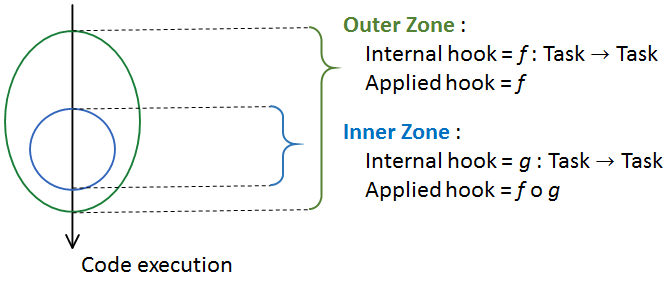
\includegraphics[width=0.7\textwidth]{around-hook}
  \caption{Around hook}
  \label{fig:around-hook}
\end{figure}

\subsection*{Around Hooks Inheritance}

For more flexibility, around hooks are inherited but not repeated. Consider three zones :

\begin{tabular}{|l|l|l|l|}
\hline
\textbf{Zone} & \textbf{Enclosing Zone} & \textbf{Defined hook} & \textbf{Applied hook}
\\\hline
outer Zone & None & $f$: Task $\rightarrow$ Task & $f$
\\\hline
middle Zone & outerZone & $g$: Task $\rightarrow$ Task & $f \circ g$
\\\hline
inner Zone & middleZone & $f$: Task $\rightarrow$ Task & $f \circ g$
\\\hline
\end{tabular}

In inner Zone, $f$ hook does not get applied one more time, because it would repeat inherited f hook from outer Zone. When the same hook is inherited multiple times, the outermost origin determines its application position. In the previous example, inner Zone applies $( f \circ g )$ and not $( g \circ f )$ because the outermost origin of $f$ (outer Zone) encloses the outermost origin of $g$ (middle Zone). This prevents inner Zones from modifying accidentally inherited hooks application order.

This inheritance policy is simply more general than a blind straight-forward application of all hooks. It is easy (especially programmatically) to re-create a different instance of a hook with the same functionality to prevent it from being filtered out. On the other hand, given a single function composed of many hooks, it is hard, if not impossible, to filter out repetitions to get this union-inheritance.

\section{Realisation}

The hypothesis that any submitted asynchronous code can be hooked permits to safely ignore the Zone integration when discussing its functionalities. The integration will be always possible. This is a great benefit, since it effectively decouples the Zone functional specification from its integration concerns, confronted to the multity of evoluting asynchronous frameworks in Java.

To integrate a Zone in a program, one can see it as a generalization of a Java thread local\footnote{A Java thread local is a field that is unique for each thread}. Note that the concept of thread local is not limited to Java. Indeed, it can be easily implemented using a mapping with threads as keys and thread locals as values.

When using a thread pool, the concept of thread local becomes limited, even erroneous. Thread locals are bound to a specific thread, but the user does not controls how its tasks are bound to the threads. The common pattern to solve this is to wrap submitted code with instructions that update the thread local for the code.
\begin{lstlisting}

ThreadLocal<T> threadLocal = ...
Executor executor = ...

/*
 * Submitted code will update
 * the thread local on execution.
 */
public void submitWithLocal(Runnable code, T local) {
  Runnable newCode = () -> {
    threadLocal.set(local);
    code.run();
  };

  executor.execute(newCode);
}
\end{lstlisting}

The Zone is a generalization of this method. Rather than binding a runnable, any code is accepted, denoted as \emph{task}. A task is executable code, with optionally inputs and outputs. The Zone handles internally the thread local to store itself and simply exports a bind method.
The Zone takes advantage of this binding operation to apply its internal mechaninc and all submission hooks that it defines. Based on this single binding, it provides:
\begin{itemize}
\item Asynchronous persistent context.
\item Modelled execution flow between the Zones.
\item Flexible programmable hooks on Zone transitions and code submission to the Zone.
\item Extension and reusability mechanisms to extend and implement more Zone features.
\end{itemize}


This pattern efficiently decouples the Zone integration from its functionalities. To use it, one only needs to bind each submitted asynchronous task to the Zone. This can be even simpler using a ``Zone-aware executor'', see chapter \ref{ch:impl}.

Chapter \ref{ch:asyncworld} showed that in Java, one cannot assume a single execution framework. The presented binding solution is not a uniform solution that automagically works in any context. It describes a single operation to execute on every asynchronous submission, which can even be modularized in the execution framework. That is how the Zone gets integrated in programs.


\section{Applications} % Independent chapter ?: Answer to motivation.

So far, the presented Zone is mostly theoretical. Around and crossing hooks have a precisely defined behavior, but beside Zone local storage, no feature answers the motivations for the Zone. I show here how to combine the Zone properties to build solution the initial problems.

\subsection*{Asynchronous error handling}

Asynchronous error handling exists in two forms, contextual and systematic.

\paragraph{The contextual error handling} consists in using the Zone as a standard try-catch block. The figure \ref{fig:sas-tc} illustrates the parallel between synchronous and asynchronous error handling.

In this example, \lstinline{future = asyncCall()} starts an asynchronous task and return the \lstinline{Future} result of that task. Of course, the task will throw an error. Two cases are considered.

\begin{enumerate}
\item Access \lstinline{message} inside the \lstinline{ErrorZone}\\
The error is not handled by the \lstinline{ErrorZone}. Nothing gets printed, since \lstinline{future.get()} synchronously throws its error inside the \lstinline{ErrorZone}.
\item Access \lstinline{message} outside the \lstinline{ErrorZone}\\
Upon \lstinline{future.get()}, the result, zoned inside \lstinline{ErrorZone} must cross out the Zone. The error gets handled and a fallback value is provided.
\end{enumerate}

The \lstinline{ErrorZone} simply has to implement the crossing hook:

\begin{lstlisting}
/*
 * Checks if crossing token 'token' is an error token.
 * If yes, handle the error.
 */
public Token crossOut(Token token) {
  if (token.isErrorToken()) {
    Token fixed;
    // error handling ...
    return fixed;
  } else {
    // do nothing
    return token;
  }
}
\end{lstlisting}

The cross resolution algorithm then accomplishes the work of selecting correct hooks according to the calling context.

\begin{figure}[H]
\centering
\makebox[0pt][c]{
\begin{minipage}[l]{0.6\linewidth}
\centering
\begin{lstlisting}
Future<String> future;^^J
^^J
// begin of async try-catch block^^J
(new ErrorZone()).run(() -> {^^J
^^J
\ \ future = asyncCall();^^J
^^J
\ \ // (1)^^J
\ \ String message = future.get();^^J
\ \ System.out.println(message);^^J
});^^J
// end of async try-catch block^^J
^^J
// (2)^^J
String message = future.get();^^J
System.out.println(message);^^J
\end{lstlisting}
\end{minipage}


\begin{minipage}[c]{0pt}
\begin{center}
\rule{0.4mm}{0.3\textheight}
\end{center}
\end{minipage}

\begin{minipage}[r]{0.6\linewidth}
\centering
\begin{lstlisting}
String future;^^J
^^J
// begin of sync try-catch bloc^^J
try {^^J
^^J
\ \ message = syncCall();^^J
^^J
\ \ // (1)^^J
\ \ System.out.println(message);^^J
^^J
} catch (Error e) { ... }^^J
// end of sync try-catch block^^J
^^J
// (2)^^J
^^J
System.out.println(message);^^J
\end{lstlisting}
\end{minipage}
}
\caption{Asynchronous and synchronous try-catch block}
\label{fig:sas-tc}
\end{figure}

\paragraph{Systematic error handling} is an automatization to uniformly wrap asynchronous code \emph{inside} a try-catch block. This can be compared to Java's \lstinline{Thread.UncaughtExceptionHandler} with the differences:

\begin{enumerate}
\item The code catches the errors \emph{before} some third-party execution service (thread pool for example), preventing the exeuction to reach the \lstinline{Thread.UncaughtExceptionHandler}.
\item The setting is not global but local to the zoned portion of the code. With \lstinline{Thread.UncaughtExceptionHandler}, one has to carefully set and unset the value.
\item Many different default exception handler can be easily emitted by the same thread.
\end{enumerate}

Such behavior is provided by a Zone implementing the asynchronous hook:

\begin{lstlisting}
// asynchronous hook
ZonedTask aroundSubmit(ZonedTask task) {
  return (input) -> {
    ZonedToken result = task.apply(input);
    if (result.isErrorToken()) {
      ZonedToken fallbackValue;
      //handle logic, compute fallbackValue
      return fallbackValue;
    } else {
      return result;
    }
  };
}
\end{lstlisting}

Since around hooks completely apply before crossing out the Zone, cross-out based error handling does not interfere with this code.

\subsection*{One Zone per asynchronous task}

This is not a direct solution to one problem of chapter \ref{ch:motivs}, but an intermediate tool to build other features. The idea is simple. Use an asynchronous hook to bind submitted task inside a new Zone.

\begin{lstlisting}
ZonedTask aroundSubmit(ZonedTask task) {
  Zone newZone = new ZoneX();
  ZonedTask newTask = newZone.bind(task);
  return newTask;
}
\end{lstlisting}

\lstinline{ZoneX} can be any Zone implementation, with the single constraint that it should override the internal hook application mechanism to do nothing. Otherwise, \lstinline{newTask} may apply unexpected internal hooks, inherited by enclosing Zones. The problem is that any \emph{internal} hooks will be also applied where \emph{asynchronous} hooks are.

\subsection*{Long stack traces}

Implementation of long stack traces use one Zone per asynchronous task to set a Zone value containing the call stack trace of the asynchronous task. With contextual error handling, it simply defines an asynchronous hook to run submitted code inside a new Zone that:
\begin{enumerate}
\item Stores as Zone local value the stack trace at the asynchronous submission.
\item Wraps zoned code inside a try-catch block to catch any error, append stored stack trace and re-throw it.
\end{enumerate}

Long stack traces are also possible with systematic error handling, but require heavier mechanisms to ensure that the stack trace is always updated before being caught by the \lstinline{catch} clauses of error handling.

\subsection*{Asynchronous dependency tracing}

Chapter \ref{ch:inpractice} discusses in details asynchronous dependency tracking as a concrete experiment. The principle is however simple. Use one Zone per asynchronous task with IDs and implement a crossing hook to store the transitions from one Zone to another one to some data structure of your choice. One Zone per task creates a one-to-one correspondance between asynchronous tasks and IDs, the crossing hook detects and stores execution dependencies between two IDs.
